 \\\documentclass[sigconf]{acmart}

\input{format/final}

\begin{document}
  \title{Comparing Predictive Models of Pain Reliever Misuse and Abuse}
  \author{Sean M. Shiverick}
  \affiliation{
  \institution{Indiana University-Bloomington}
  }
\renewcommand{\shortauthors}{S.M. Shiverick}

%%%%%%%%%%%%%%%%%%%%%%%%%%%%%%%%%%%%%%%%%%%%%%%%%%%%%%%%%%%%%%%%%%%%%%%%%%%%%%%%

\begin{abstract}

Prescription opioid abuse and addiction is a chronic health condition that 
has resulted in increased overdose deaths in recent years \cite{nida18}. 
Predictive modeling can identify factors related to MUPO and may help predict 
individuals at risk for opioid addiction. The present study compares several 
linear and non-linear classification models of pain reliever misuse and abuse 
and considers advantages and limitations of the different models. The sample 
data consisted of N = 114,038 respondents from the National Survey on Drug Use 
and Health (NSDUH) for 2015 and 2016. Classifier models were fit to a training 
set, class labels were predicted for holdout observations in the test set, and 
model performance was evaluated in a confusion matrix. 

[Summarize findings]

Simple models had lower accuracy but provide more interpretable solutions 
than complex models which can yield higher accuracy but are often harder 
to interpret.   

\footnote{ Address correspondence to \textit{smshiver@iu.edu}}
\end{abstract}
\keywords{Predictive Modeling, Supervised Learning, Classification Models}
\maketitle

%%%%%%%%%%%%%%%%%%%%%%%%%%%%%%%%%%%%%%%%%%%%%%%%%%%%%%%%%%%%%%%%%%%%%%%%%%%%%%%%
\section{Introduction}

Over the past two decades the misuse and abuse of prescription opioids (MUPO)  
has become a major health crisis in the U.S. \cite{volkow14}. In 2015, an 
estimated 2 million Americans suffered a substance use disorder related 
to prescription opioid pain relievers such as oxycodone or hydrocodone 
in 2015 \cite{nida18}. Opioid dependence and relapse are chronic health 
conditions and following treatment many addicted individuals are at high 
risk for relapse and overdose death \cite{shaham03}. The number of opioid-
related overdose deaths has more than quadrupled from 1999 to 2016. 
Each day, an average of 115 people die from an opioid overdose in the U.S. 
\cite{cdc18, judd16}. Supply-based interventions to reduce the availability 
of prescription opioids have produced a shift to the use of heroin and 
synthetic opioids such as fentanyl \cite{jones15}. The risk of overdose 
death from illicit and synthetic opioids is greatly increased because 
the dosage levels and potency are largely unknown. The sharp rise in 
prescription overdose deaths (POD) and heroin overdose deaths (HOD) are 
correlated \cite{muhuri13, unick13}. Predictive modeling approaches can 
help identify individuals susceptible for opioid addiction and may provide 
insights that inform policy decisions for addressing the opioid crisis. 
This study compares different classification models of pain reliever misuse 
and abuse and identifies several important features that contribute to 
the misuse and abuse of prescription opioids. 

%%%%%%%%%%%%%%%%%%%%%%%%%%%%%%%%%%%%%%%%%%%%%%%%%%%%%%%%%%%%%%%%%%%%%%%%%%%%%%%%

\subsection{Predictive Modeling}

Predictive modeling, statistical learning, or machine learning describe a 
set of procedures and automated processes for extracting knowledge from data 
\cite{james13, kuhn13, muller17, raschka17}. The two main branches of 
predictive modeling are supervised learning and unsupervised learning. 
Supervised learning problems involve prediction about a specific target 
variable or outcome. If a given dataset has no target outcome, unsupervised 
learning methods can be used to discover underlying structure in unlabeled data 
(e.g., clustering). Supervised learning is used to predict a certain outcome 
from a given input, when examples of input/output pairs are available in the 
data (e.g., logistic regression) \cite{muller17}. A statistical learning model 
is constructed on a set of observation used to train the model set and can then 
be used to predict new observations. Two major approaches to supervised learning 
problems are regression and classification. When the target variable to be 
predicted is continuous, or there is continuity between the outcome 
(e.g., home values), a regression model is used to test the set of features 
that predict the target variable. If the target is a class label, set of 
categorical or binary outcomes (e.g., spam or ham emails, benign or malignant 
cells), then classification is used to predict which class or category label 
that new instances will be assigned to. The present study uses a supervised 
learning approach to classify instances of pain reliever misuse and abuse 
using several classification models. 

%%%%%%%%%%%%%%%%%%%%%%%%%%%%%%%%%%%%%%%%%%%%%%%%%%%%%%%%%%%%%%%%%%%%%%%%%%%%%%%%

In the era of ``big data'', large amounts of health information are being 
generated from electronic medical records (EMRs), clinical research data, to 
population-level health data \cite{herland14}. It can be difficult to obtain 
reliable information about drug use based on self-reports, though surveys 
provide data on a range of issues that people may be reluctant to disclose 
such as drug use and mental health problems. This study considers data from 
the National Survey on Drug Use and Health (NSDUH) which is a major source of 
information for the use of illicit drugs and mental health issues among the 
U.S. population aged 12 or older \cite{samhsa18}. The NSDUH is a comprehensive 
public survey that includes more than 2600 variables on a diverse array of 
questions related to the use, misuse, and abuse of substances including 
alcohol, tobacco, prescription medications, and illicit drugs. In addition 
to typical demographic information, the survey includes self-reported 
measures on items related to physical health, mental health (e.g., depression, 
anxiety, suicidal ideation), counseling, and drug and alcohol treatment. 
Data from the NSDUH has been used for identifying groups at high risk for 
substance use, and the co-occurrence of substance use and mental health 
disorders. The target variable for the study was any misuse or abuse of 
prescription pain relievers and the features of interest were selected 
demographic variables, medication usage, and use of illicit drugs. 

%%%%%%%%%%%%%%%%%%%%%%%%%%%%%%%%%%%%%%%%%%%%%%%%%%%%%%%%%%%%%%%%%%%%%%%%%%%%%%%%

\subsection{Classification Models}

\subsubsection{Linear Classifier Models}

As stated by statistician George Box, "All models are wrong, but some models 
are useful" \cite{box05}. There are advantages and limitations for using any 
classification model, but logistic regression is one of the most useful,
reliable, and interpretable models to select from. Logistic regression models 
the conditional distribution of probabilities for a binary response (e.g., 
$Pr(Y=k | X=x)$) as a combination of a set of predictor variables 
\cite{james13, raschka17}. The decision boundary for the logistic regression 
classifier is a linear function of the input; a binary classifier separates 
two classes using a line, plane, or hyperplane \cite{muller17}. Given that the 
probability values for the outcome range between 0 and 1, predictions can be 
made based on a default value. For example, a default value of `Yes` could be 
predicted for any individual for whom the probability of pain reliever misuse 
and abuse is greater than fifty-percent, $Pr(PRLMISAB) > 0.5$. Logistic regression 
uses a maximum likelihood method to predict the coefficient estimates that 
correspond as closely as possible to the default state. In other words, the 
model will predict a number close to one for individuals who have misused or 
abused pain relievers and a number close to zero for individuals who have 
not. The distribution of conditional probabilities in the logit model has an 
S-shaped curve. The coefficients estimates obtained from a logistic regression 
model, ($beta_0$, $beta_1$ ... $beta_k$) are selected in order to maximize the 
likelihood function, and are interpreted as an indication of the log-odds 
change in the outcome variable that is associated with a one-unit increase 
in a predictor variable ($X_i$...$X_j$). 

%\begin{figure}[!ht]
%  \centering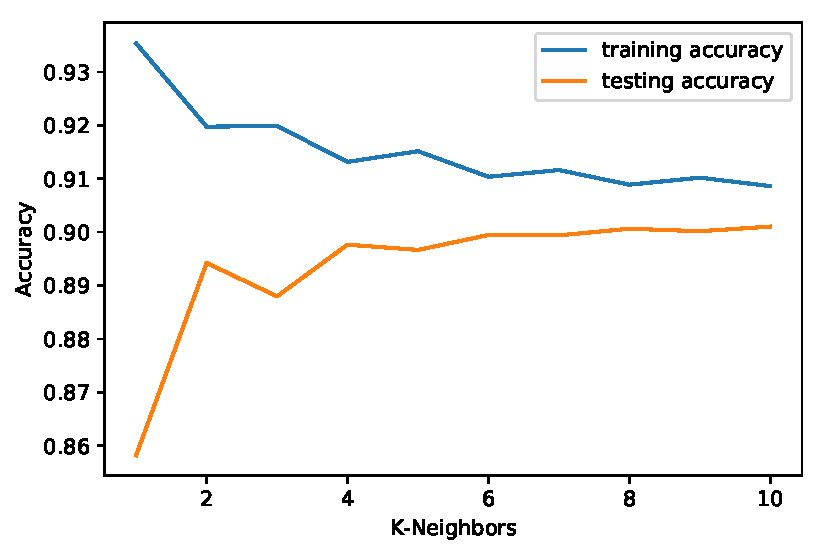
\includegraphics[width=\columnwidth]{images/Figure2.pdf}
%  \caption{Conditional Probabilities for Predicting Class Labels with 
%  a Logistic Regression Model \cite{raschka17}}
%  \label{f:Figure2}
%\end{figure}

\emph{Linear discriminant analysis} (LDA) is an alternative approach to 
estimating the probabilities which models the distribution of predictors 
separately in each of the response classes and then uses the Bayes' theorem 
to flip these into estimates for $Pr(Y=k | X=x)$ \cite{james13}. The term 
linear in LDA refers to the the discriminant functions being linear functions 
of the predictors. For distributions assumed to be normal (i.e., multivariate 
Guassian), LDA provides a model that is similar in form to logistic regression, 
but more stable. LDA is also preferred for outcomes with more than two response 
classes. Two important assumptions of LDA are: (1) a common covariance matrix 
for all classes and (2) the class boundaries are linear functions of the 
predictors. \emph{Quadratic Discriminant Analysis} (QDA) is an approach that 
assumes each class has its own covariance matrix and the decision boundaries 
are quadratically curvilinear in the predictor space \cite{kuhn13}. LDA is less 
flexible as a classifier than QDA, but can perform better with relatively few 
training observations or when the majority of predictors in the data represent 
discrete categories. QDA is recommended over LDA with a very large training 
set or when the decision boundary between two classes is non-linear. 

%%%%%%%%%%%%%%%%%%%%%%%%%%%%%%%%%%%%%%%%%%%%%%%%%%%%%%%%%%%%%%%%%%%%%%%%%%%%%%%%

\subsubsection{Non-linear Classifier Models}

The performance of linear classifiers suffers when there is a non-linear 
relationship between the predictors and target outcome. With training
observations that can be separated by hyperplane, the maximal marginal 
classifier provides the maximum distance (i.e., margin) from each observation
to the hyperplane \cite{james13}. The test observations are classified based 
on which side of the hyperplane they fall, but in many cases no separating 
hyperplane exists. The \emph{support vector classifier} (SVC) extends the 
maximal margin classifier by using a soft margin that allows a small number 
of observations to be misclassified on the wrong side of hyperplane 
\cite{kuhn13, cortes95}. The observations that fall directly on the margin or 
on the wrong side of the hyperplane are called `support vectors'. The parameter 
`C' indicates the number of observations that can violate the margin; if $C>0$, 
no more than C observations can be on the wrong side of the hyperplane. 
SVC addresses the problem of non-linear boundaries between classes by 
enlarging the feature space with higher order (e.g., quadratic, cubic, 
polynomial) functions of the predictors. 

\begin{figure}[!ht]
  \centering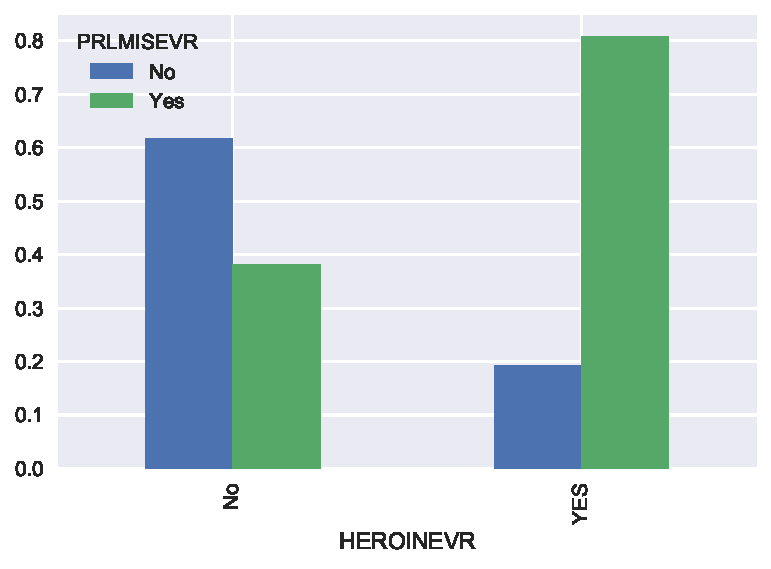
\includegraphics[width=\columnwidth]{images/Figure3.pdf}
  \caption{Decision Boundary and Support Vectors for Support Vector Machine 
  SVM Classifier with Nonlinear Kernel \cite{muller17}}
  \label{f:Figure3}
\end{figure}

\emph{Support vector machines} (SVM) are an extension of SVC that use a 
kernel trick to reduce computational load. The radial basis function (RBF) 
kernel (i.e., Guassian kernel) is one of the most commonly used approaches. 
In training the model, only a subset of data points is used to construct the 
decision boundary, namely the support vectors that lie on the border that 
separates the two classes. In making predictions for new observations, the 
algorithm calculates the distance to each of the support vectors measured by 
the Guassian kernel \cite{muller17}. Figure 1 shows an example of the non-linear 
decision boundary obtained with SVM using the RBF kernel; the decision boundary 
is a smooth curve and the support vectors are the large points in bold outline. 
With the default settings, the decision boundary of the RBF kernel is already 
non-linear. The main parameters for SVM are `C', which regulates the importance 
of each data point, and `gamma' which controls the width of the Guassian kernel. 
A small value of C indicates a restricted model in which the influence of each 
data point is limited and the algorithm adjusts to the majority of data points. 
With larger values of C, more importance is given to each data point and the 
model will try to correctly classify as many training observations as possible, 
which results to more curve in the decision boundary, but also increases the 
risk of overfitting to the training data. Large values of gamma mean that only 
close values are relevant for classification, resulting in a smooth decision 
boundary. Small values of gamma mean that far points are similar. If the values
of both C and gamma are large, each point can have an arbitrary large influence 
in a small region, which produces a choppy decision boundary, where each point 
becomes separated as its own class. If both C and gamma are small, the decision 
boundary becomes close to linear.

%%%%%%%%%%%%%%%%%%%%%%%%%%%%%%%%%%%%%%%%%%%%%%%%%%%%%%%%%%%%%%%%%%%%%%%%%%%%%%%%

The Bayes' rule was mentioned above in relatin to LDA, but this section 
considers the \emph{naive Bayes classifier} as a non-linear model.
The Bayes theorem (equation 2) is represented by a set of probabilities to 
represent the following question: Based on a given set of predictors, what
is the probability than an outcome belongs to a particular class?

\begin{equation}
  \ P(Y=cl|X) = \frac{P(Y)*P(X|Y=cl)}{P(X)}\
\end{equation}

The prior probability, P(Y), is the expected probability of a given class 
based on what is known (e.g., rate of disease in the population). P(X) 
is the probability of the predictor variables. The conditional probability,
$P(X=cl|Y)$, is the probability of observing the predictor variables for data 
associated with a given class. The naive Bayes model is based on the 
assumption that all the predictor variables are independent, although this 
is not always realistic. The conditional probabilities are calculated based 
on the probability densities for each individual predictor \cite{kuhn13}. 
For categorical predictors, the observed frequencies in the training set data 
can be used to determine the probability distributions. The prior probability 
allows us to tilt the final probability toward a particular class. Class 
probabilities are created and the predicted class is one associated with the 
largest class probability. Despite the somewhat unrealistic assumption of 
independence among predictors, the naive Bayes model is computationally quick, 
even with large training sets, and performs competitively compared to other 
models. The naive Bayes model encounters issues when dealing with frequencies 
or probabilities equal to zero, especially for small sample sizes. In addition, 
as the number of predictors increases relative to sample size, the posterior 
probabilities will become more extreme.

%%%%%%%%%%%%%%%%%%%%%%%%%%%%%%%%%%%%%%%%%%%%%%%%%%%%%%%%%%%%%%%%%%%%%%%%%%%%%%%%

\emph{Neural Networks} are powerful models for classification and 
regression based on theories about connectivity in the brain \cite{kuhn13}. 
The pstudy considers a simple method called multilayer perceptrons 
(MLP) as a feed-forward neural network \cite{muller17, raschka17}. 
The outcome is modeled by an intermediary set of unobserved variables called 
hidden units, which are linear combinations of the original predictors. 
Each hidden unit is a combination of some or all of the predictors which 
are then transformed by a nonlinear function (e.g., sigmoidal). A neural 
network usually has multiple hidden units used to model the outcome. 
The MLP classifier computes weights between the inputs and the hidden layers, 
and weights between the hidden layers and the output. After computing each 
hidden unit, the output is modeled by a nonlinear combination of the hidden 
units. The nonlinear function allows the neural network to fit more 
complicated functions than a linear model. Neural networks are sensitive to 
the scaling of the features and can require extensive data preprocessing. 
There are several ways to modify the complexity of a neural network: by 
selecting the number of hidden layers, the number of units within each 
layer, and the regularization parameter (L2) which shrinks the weights 
towards zero. The feature weights provide an estimate of feature importance.
Although neural networks can capture information in large amounts of data 
with very complex models, some limitations are that they tend to overfit 
data used to train the model, and can be difficult to interpret. Neural
networks may work best with homogenous datasets where the predictor variables
all have similar meanings \cite{muhuri13}. For datasets with many different
kinds of features, tree-based methods may provide a better approach.

%%%%%%%%%%%%%%%%%%%%%%%%%%%%%%%%%%%%%%%%%%%%%%%%%%%%%%%%%%%%%%%%%%%%%%%%%%%%%%%%

\subsubsection{Tree-based Models} Decision trees are based on a hierarchy of 
\emph{`if-else'} questions starting from a root node and proceeding through a 
series of binary decisions or choices. Each node in the tree represents either 
a question or a terminal node (i.e.,leaf) that contains the outcome. Applied to 
a binary classification task, the decision tree algorithm learns the sequence
of if-else questions that arrives at the outcome most quickly. For continuous 
features, questions are expressed in the form: ``Is feature x larger than 
value y?'' In constructing the tree, the algorithm searches through all 
possible tests and finds a solution that is most informative about the target 
outcome \cite{muller17}. The recursive branching process yields a binary tree 
of decisions, with each node representing a test for a single feature. This 
process of partitioning is repeated until each leaf in the decision tree 
contains only a single target. Prediction for a new data point proceeds by 
checking which region of the partition the point falls in, and predicting the 
majority in that feature space. The main advantage of tree models is that they 
require little adjustment and are easy to interpret. A drawback is that they 
can lead to complex models which are highly overfit to the training data. 
Prepruning`can help reduce overfitting by limiting the maximum depth of the 
tree, or the maximum number of leaves. Another approach is to set the minimum 
number of points in a node required for splitting. Decision trees work well 
with features measured on different scales, or with data that has a mix of 
binary and continuous features. 

%%%%%%%%%%%%%%%%%%%%%%%%%%%%%%%%%%%%%%%%%%%%%%%%%%%%%%%%%%%%%%%%%%%%%%%%%%%%%%%%

\emph{Random Forests} is an ensemble approach that combines many simple trees 
that each overfit the data in different ways. By building many trees and 
averaging their results, random forests helps to reduce overfitting. In 
constructing the forests, the user selects the number of trees to build 
(e.g., 1000). Randomness is introduced using a bootstrapping method that 
repeatedly draws random samples of size n from the data set (with replacement).  
The decision trees are build on these random samples of the same size, with 
some points missing and some data points repeated \cite{muller17,raschka17}.
The algorithm makes a random selection of p- features, and uses a different 
set of features at each node branch. These processes ensure that all of the 
decision trees in the random forest are different. Random forests is one of 
the most widely used supervised learning algorithms that works well without 
very much parameter tuning or scaling of data. A limitation is that Random 
forests do not perform well with high-dimensional data, or data that is 
sparse such as text data.

%%%%%%%%%%%%%%%%%%%%%%%%%%%%%%%%%%%%%%%%%%%%%%%%%%%%%%%%%%%%%%%%%%%%%%%%%%%%%%%%

\emph{Gradient Boosted trees} is another ensemble method that combines 
multiple decision trees in a serial fashion, where each tree tries to correct 
for mistakes of the previous one \cite{muller17}. Gradient boosted regression 
trees use strong pre-pruning, with shallow trees of a depth of one to five. 
Each tree only provides a good estimate of part of the data; combining many 
shallow trees (i.e., ``weak learners'') iteratively improves performance. 
In addition to pre-pruning and the number of trees, an important parameter 
for gradient boosting is the \emph{learning rate} which determines how strongly 
each tree tries to correct for mistakes of previous trees. A high learning rate
produces stronger corrections, allowing for more complex models. Adding more 
trees to the ensemble also increases model complexity. Gradient boosting
and random forests perform well on similar tasks and data. A common 
approach is to first try random forests and then include gradient boosting 
to improve model accuracy. 

%%%%%%%%%%%%%%%%%%%%%%%%%%%%%%%%%%%%%%%%%%%%%%%%%%%%%%%%%%%%%%%%%%%%%%%%%%%%%%%%

\subsection{Metrics for Evaluating Prediction Models}

Evaluating the performance of learning algorithms is helpful for selecting 
the best model for a given problem and data set. Binary classification is 
assessed in terms of the successful assignment of observations to one of two 
classes: positive or negative. Medical testing outcomes are often used to 
illustrate classification decisions and errors. A person can be either 
diagnosed with an illness or not, and the person can actually have the 
illness or not. In the present case, individuals are classified as having 
misused and abused pain relievers or not, and the predictions made are either 
correct or incorrect. Model performance is typically evaluated using accuracy 
which is the number of correct predictions divided by the total number of 
all samples. Any model selected cannot make perfect predictions as there are 
always mistakes to be found. For example, a negative instance can be labeled 
as positive: a person who has never misused or abused pain relievers may be 
classified as having done so (i.e., 'false positive'). Conversely, a positive 
instance may be classified as negative: a person who has misused and abused 
pain relievers may be labeled as never having done so (i.e., 'false negative').

%%%%%%%%%%%%%%%%%%%%%%%%%%%%%%%%%%%%%%%%%%%%%%%%%%%%%%%%%%%%%%%%%%%%%%%%%%%%%%%%

\begin{table}
  \caption{Confusion Matrix for Evaluating Classification Model Performance}
  \label{tab:freq}
  \begin{tabular}{llll}
    \toprule
     &  &  Actual Outcome & \\
    \midrule
     Predicted & Outcome & No Misuse & PRL Misuse \\
    \midrule
     & No Misuse & \textbf{True Negative} & False Positive \\
    \midrule
     & PRL Misuse & False Negative & \textbf{True Positive} \\
    \bottomrule
  \end{tabular}
\end{table}

Classification errors and correct decisions can be represented in a 
\emph{confusion matrix} (Table 1) that indicates the correspondence between 
predicted and actual outcomes. The confusion matrix is a two-by-two array in 
which the columns correspond to the actual observed classes and the rows 
correspond to the predicted classes. The main diagonal indicate the number of 
correctly classified samples (\emph{true positive, true negative}, while the 
other entries represent the number of samples in one class that were mistakenly 
classified as another class. Classification models are evaluated using several 
measures including recall, precision, and the $f_1$-score \cite{wiki18}. 
\emph{Recall} or ``sensitivity'' measures how many positive samples are 
captured by the positive predictions ( \(\frac{TP}{TP+FN}\) ), and is used 
when we want to identify all positive samples while avoiding false negatives. 
\emph{Precision} or the ``positive predictive value'', measures how many of 
the samples predicted as positive are actually positive  
( \(\frac{TP}{TP+FP}\) ), and is used as a metric when the goal is to limit 
the number of false positives. The \emph{$f_1$-score} or `f-measure' provides 
the harmonic mean of precision and recall. The $f_1$-score can be a better 
metric than accuracy in datasets with \emph{imbalanced classes}, where one 
class is much more frequent than the other class, as it takes recall and 
precision into account \cite{muller17}.

\begin{equation}
  \ f_1 score = 2*\frac{Precision*Recall}{Precision+Recall}\
\end{equation}

 \begin{figure}[!ht]
  \centering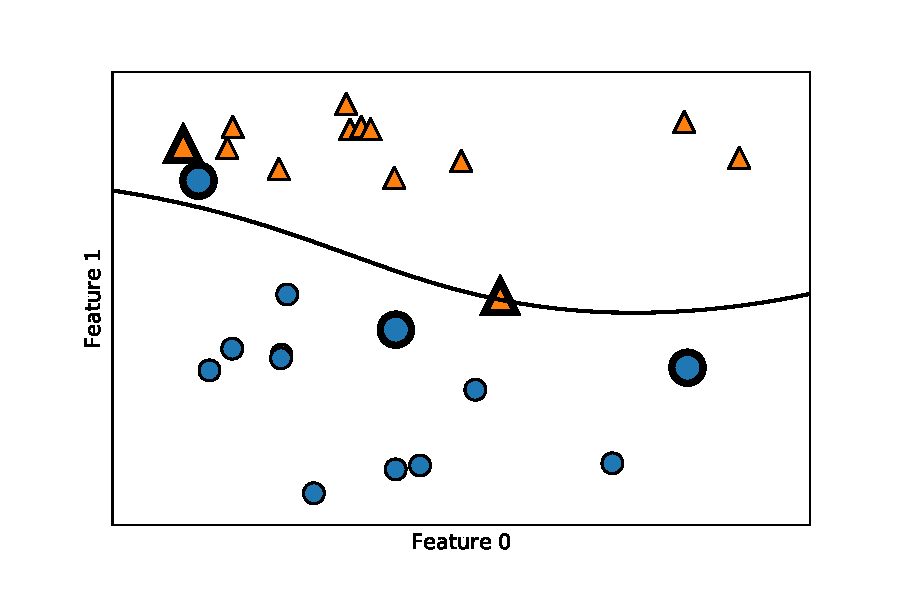
\includegraphics[width=\columnwidth]{images/Figure1.pdf}
  \caption{K-Nearest Neighbors Classifier Accuracy for Training Set and 
  Testing Set as a function of Number of Neighbors}
  \label{f:Figure1}
\end{figure}

%%%%%%%%%%%%%%%%%%%%%%%%%%%%%%%%%%%%%%%%%%%%%%%%%%%%%%%%%%%%%%%%%%%%%%%%%%%%%%%%

\subsubsection{Training and Test Set Accuracy}

In constructing and evaluating predictive models it is important to select 
a model that performs well not only with data used to train the model, but 
also with new observations that are previously `unseen'. The sample data
is divided into two portions: a \emph{training set} used to fit the model 
and a \emph{testing set} of observations that is set aside and used to 
evaluate model performance. By convention, approximately 70 to 80 percent of 
observations are used in the training set and the remaining observations 
are held in the testing set. Two main problems can occur in evaluating model 
performance: overfitting and underfitting. In the case of \emph{overfitting}, 
a model can have high accuracy on the training set but perform poorly with 
new data in the test set because the model is `over-fit' to the training data, 
By contrast, ``underfitting'' occurs when a model performs poorly with the 
training data but has higher accuracy with the new observations in the test 
set. One of the simplest predictive models, K-Nearest neighbors, classifies 
observations by assigning the label that is most frequent among the `k' number 
of nearest training samples. K is a parameter selected by the user. The 
accuracy of the KNN classifier for the training set and testing set is 
plotted as a function of the parameter k-neighbors in Figure 1. The plot 
shows a tradeoff in training accuracy versus testing accuracy; higher accuracy
on the testing set is associated with a slight decrease in performance on the
training set. The best model is one that optimizes testing set accuracy, 
while striking a balance between the problems of overfitting and underfitting.
In this case, performance on the test set increased slightly between 2 and 4 
neighbors, but does not improve much beyond 5 neighbors. Therefore, a KNN
model with k=4 neighbors will provide a reasonable solution for the data. 

%%%%%%%%%%%%%%%%%%%%%%%%%%%%%%%%%%%%%%%%%%%%%%%%%%%%%%%%%%%%%%%%%%%%%%%%%%%%%%%%

\begin{table*}[ht]
  \caption{Summary of Variables in the NSDUH 2015-16 Aggregated Data Set}
  \label{tab:freq}
  \begin{tabular}{ll}
    \toprule
    \textit{Target Outcome} & Label \\
    \midrule
    Prescription Opioid Pain Reliever Misuse and Abuse (Likert scale: 0-12)& PRLMISAB  \\
    \midrule
    \textit{Predictor Variables}&   \\
    \midrule
    Age Category (1=12-17 years, 2=18-25, 3=26-34, 4=35-49, 5=50 and older)& AGECAT \\
    Biological Sex (0=Male, 1=Female)& SEX  \\
    Marital Status (0=Unmarried, 1=Divorced, 2=Widowed, 3=Married)& MARRIED  \\
    Education (1=H.S. or Less, 2=H.S. Grad., 3=Some College,  4=College Grad.)& EDUCAT  \\
    Size of City/Metropolitan Region (1=Rural, 2=Small, 3=Large)& CTYMETRO  \\
    Health Problems Aggregated  (Likert scale: 0-10)& HEALTH  \\
    Mental Health, Aggregated: adult depression, emotional distress (Likert scale: 0-10)& MENTHLTH  \\
    Treatment for Drugs and Alcohol in past year, Aggregated (Likert scale: 0-5)& TRTMENT  \\
    Mental Health Treatment, Aggregated (Likert scale: 1-10)& MHTRTMT  \\
    Tranquilizer use, past year, Aggregated (Likert scale: 0-5)& TRQLZRS \\
    Sedative use, past year, Aggregated (Likert scale: 0-5)& SEDATVS  \\
    Heroin use, past year, Aggregated (Likert scale: 0-5)& HEROINUSE  \\
    Cocaine and Crack Cocaine Use in past year, Aggregated  (Likert scale: 0-5)& COCAINE  \\
    Amphetamine and Methamphetamine Use in past year, Aggregated (Likert scale: 0-5)& AMPHETMN  \\
    \bottomrule
  \end{tabular}
\end{table*}


%%%%%%%%%%%%%%%%%%%%%%%%%%%%%%%%%%%%%%%%%%%%%%%%%%%%%%%%%%%%%%%%%%%%%%%%%%%%%%%%

\section{Method}

\subsection{The Data}

The NSDUH public data files for 2015 and 2016 were downloaded from the 
Substance Abuse and Mental Health Data Archive (SAMHDA) \cite{samhsa18}. 
The data sets were extracted and saved as data frame objects in a python 
interactive notebook \cite{mckinney17, vanderplas17}. The 2015 NSDUH data set 
consisted of N=57146 respondents with 2667 variables and the 2016 data set had 
N=57897 individuals and 2665 variables, resulting in a total sample of N=114043 
observations (53873 male, 60165 female). As described in the NSHUD codebook, 
the sampling design was weighted across states by population size, drawing more 
heavily from eight states with the largest populations (CA, FL, IL, MI, NY, OH, 
PA, TX), for a representative distribution that accounts for approximately 
48 percent of the U.S. population. For 2015, the weighted survey screening 
response rate  was 81.94\% and the weighted interview response rate was 71.2\% 
\cite{samhsa18}. Identifying information in the public use files is collapsed 
(e.g., age categories); variables related to ethnicity, immigration status, and 
state identifiers are removed to ensure confidentiality. The data frames were 
subset by column to select approximately 90 variables that included common 
demographic characteristics, physical health, mental health, medication usage, 
and use of illicit drugs. The following steps were taken to detect and remove 
any inconsistencies in the data: (1) Remove missing values (i.e., NaN); 
(2) Recode blanks, non-responses, or legitimate skips (e.g., 99, 991, 993) to 
zero; (3) Recode dichotomous responses (e.g., Yes=1 / No=2) so that 
`No' = 0; (4) Recode categorical variables to be consistent with amount or 
degree  (e.g., 1=`Low', 2=`Med', 3=`High'). (5) Outliers were identified 
and excluded from the data set (n=5).

%%%%%%%%%%%%%%%%%%%%%%%%%%%%%%%%%%%%%%%%%%%%%%%%%%%%%%%%%%%%%%%%%%%%%%%%%%%%%%%%

\subsubsection{Aggregated Variables}

Related variables were aggregated to create features. For example, a single 
variable `HEALTH` was created by combining scores for overall health (reverse 
scored), previous diagnosis of STDs, hepatitis, HIV, cancer, or any 
hospitalization; higher scores indicated higher level of health problems. 
A variable for mental health (MENTHLTH) aggregated responses for adult 
depression, emotional distress, suicidal thoughts or plans. Any prescription 
opioid pain medication use in the past year was assessed by combining binary 
responses for ten of the most commonly used prescription pain medications 
(e.g., Hydrocodone, Oxycodone, Tramadol, Morphine, Fentanyl, Oxymorphone, 
Demerol, Hydromorphone). The majority of questions related to substance use 
had dichotomous responses that were summed to create single measures for: 
Tranquilizers, Sedatives, Heroin, Cocaine, and Amphetamines. Because 
hallucinogens varied greatly in strength and type (e.g., marijuana, 
psilocybin, MDMA, LSD), they were not included in the analysis. Variables 
for drug treatment and mental health treatment combined responses for any 
inpatient care, outpatient care, treatment at a clinic, emergency room visits, 
or hospital stays. A measure of any previous pain reliever misuse or abuse 
combined responses for the misuse, abuse, or dependency on prescription pain 
relievers in the past year, in the past month. The target variable was a 
dichotomous measure of any previous pain reliever misuse or abuse. The 
subset data frame consisted of 20 features and 114038 observations and was 
exported to CSV file. Four variables were excluded from analysis (PRLANY, 
PRLMISAB, HEROINEVR, HALUCNG). Table 2 shows the complete list of 
variables used for predictive modeling. 

%%%%%%%%%%%%%%%%%%%%%%%%%%%%%%%%%%%%%%%%%%%%%%%%%%%%%%%%%%%%%%%%%%%%%%%%%%%%%%%%

\subsubsection{Classifier Models}

The dataset was divided into the training set and test set using a 75-25 
percent split ($n_train$=85538, $n_test$=28510). The same general procedure
was used in constructing each classification model: (i) Each model was fit to 
the training set, (ii) New values were predicted on the holdout scores in the 
testing set, and (iii) Model performance was evaluated in a confusion matrix, 
and the performance metrics|accuracy, sensitivity (i.e., recall), precision|
were obtained from the confusion matrix; the $f_1-score$ was derived from the 
values for recall and precision (equation 1). The logistic regression classifier, 
LDA, QDA, decision trees classifier, random forests classifier, gradient boosted 
classifier were constructed using the caret package. The KNN classifier, support 
vector classifier (SVC), naive Bayes classifier, and neural net (multilayer 
perceptron) were constructed using scikit-learn. The main parameter settings 
for each model are reported in Table 4. 

%%%%%%%%%%%%%%%%%%%%%%%%%%%%%%%%%%%%%%%%%%%%%%%%%%%%%%%%%%%%%%%%%%%%%%%%%%%%%%%%

\begin{table}
  \caption{Classification Models for Predict Pain Reliever Misuse 
  and Abuse and Main Parameters}
  \label{tab:freq}
  \begin{tabular}{ll}
    \toprule
    Model & Main Parameter \\
    \midrule
    K-Nearest Neighbors & Number of Neighbors = 4 \\
    Logistic Regression & Number of Features = 15 \\
    Linear Discriminant Analysis (LDA) & Number of Features = 15 \\
    Quadratic Discriminant Analysis (LDA) & Number of Features = 15 \\
    Support Vector Machines (SVM) & Kernel = linear \\
    Naive Bayes & Cost C = 0.01 \\
    Neural Network & Hidden Layers = 2 \\
    Decision Trees & Tree-Depth = 4 \\ 
    Random Forests & Number of Trees = 1000 \\
    Boosted Trees & Learning Rate = 0.01 \\ 
    \bottomrule
  \end{tabular}
\end{table}

%%%%%%%%%%%%%%%%%%%%%%%%%%%%%%%%%%%%%%%%%%%%%%%%%%%%%%%%%%%%%%%%%%%%%%%%%%%%%%%%

The Decision Tree Classifier package in Scikit-Learn was used to build the 
tree model, pre-pruning was applied with a maximum depth of 4, which means 
the algorithm split on four consecutive questions. The training set accuracy 
of the pruned tree was 0.902 and test set accuracy was 0.902. Figure 9 shows 
a partial view of the decision tree classifier of prescription opioid misuse
(the full tree is included in the BDA-Analytics-Classifier-PRL.ipynb 
notebook) \cite{classifyPRL}. 

\section{Results}

\subsection{Exploratory Data Analysis}

Of the total sample of N=114038 survey respondents from 2015-2016, 27\%
(n=30790) reported taking any pain relievers in the past year (13405 males, 
17383 females). Approximately 11\% (n=12305) of the sample disclosed that 
they had previously misused or abused prescription pain relievers at some 
point (6239 males, 6066 females). Only 2\% of individuals (n=2266) disclosed 
ever using heroin (1320 males; 946 females). Given previous findings 
that indicate a relationship between the the misuse and abuse of prescription
opioids pain and heroin use \cite{muhuri13, unick13}, the exploratory analysis 
focused on misuse or abuse of pain relievers and heroin use. Figure 1 shows 
that the proportion of pain reliever misuse and abuse was higher among 
individuals who reported using heroin than those who had not. In addition, 
pain reliever misuse and abuse and heroin use both varied by sex (Figure 3). 
Although, a greater number of females than males reported using any pain 
relievers , the left panel of figure 3 shows that more females than males
reported they had not misused or abused pain relievers compared to males; 
however, roughly equal proportions of males and females reported misusing or 
abusing pain relievers. The right panel of Figure 3 shows that a higher 
proportion of males reported using heroin than females, but more females 
reported they had never used heroin than males. 

\begin{figure}[!ht]
  \centering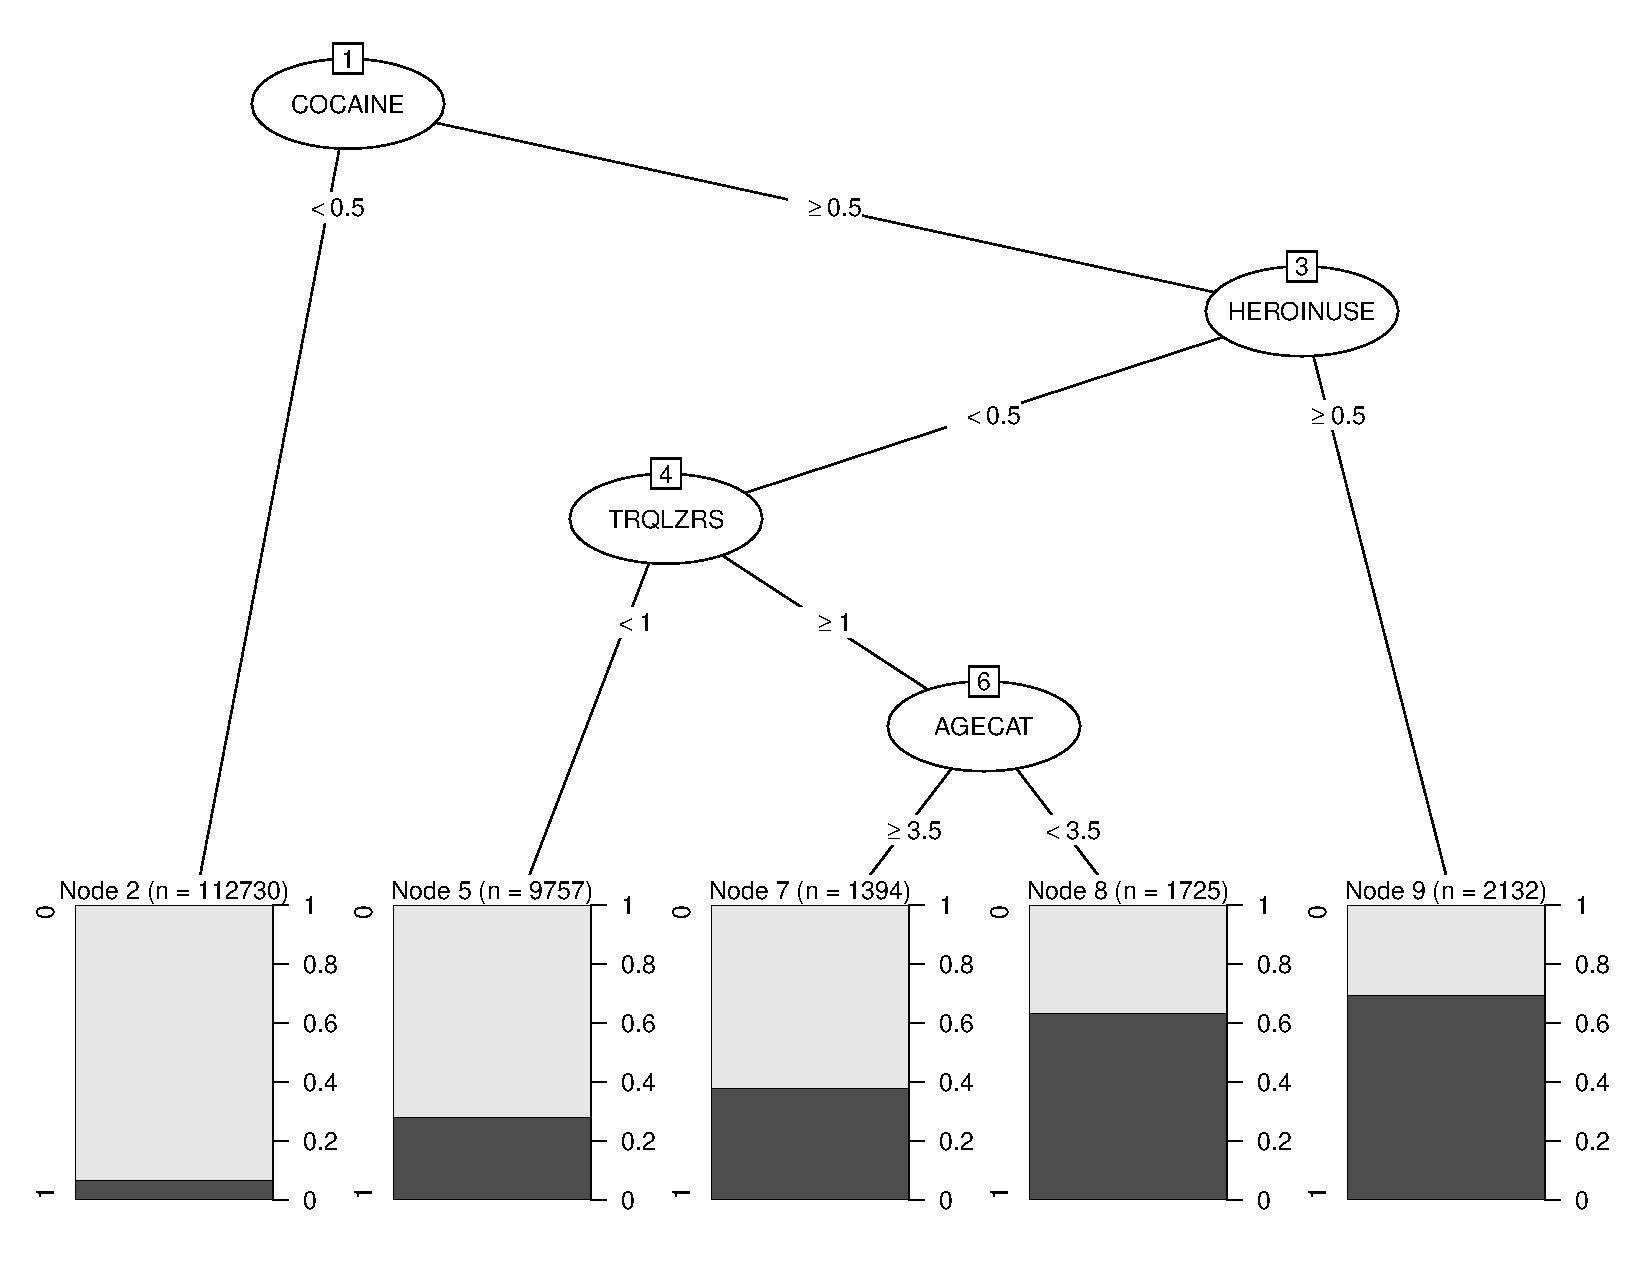
\includegraphics[width=\columnwidth]{images/Figure4.pdf}
  \caption{Proportion of Individuals Reporting Pain Reliever Misuse and Abuse
  as a function of Heroin Use Ever}
  \label{f:Figure4}
\end{figure}

\begin{figure}[!ht]
  \centering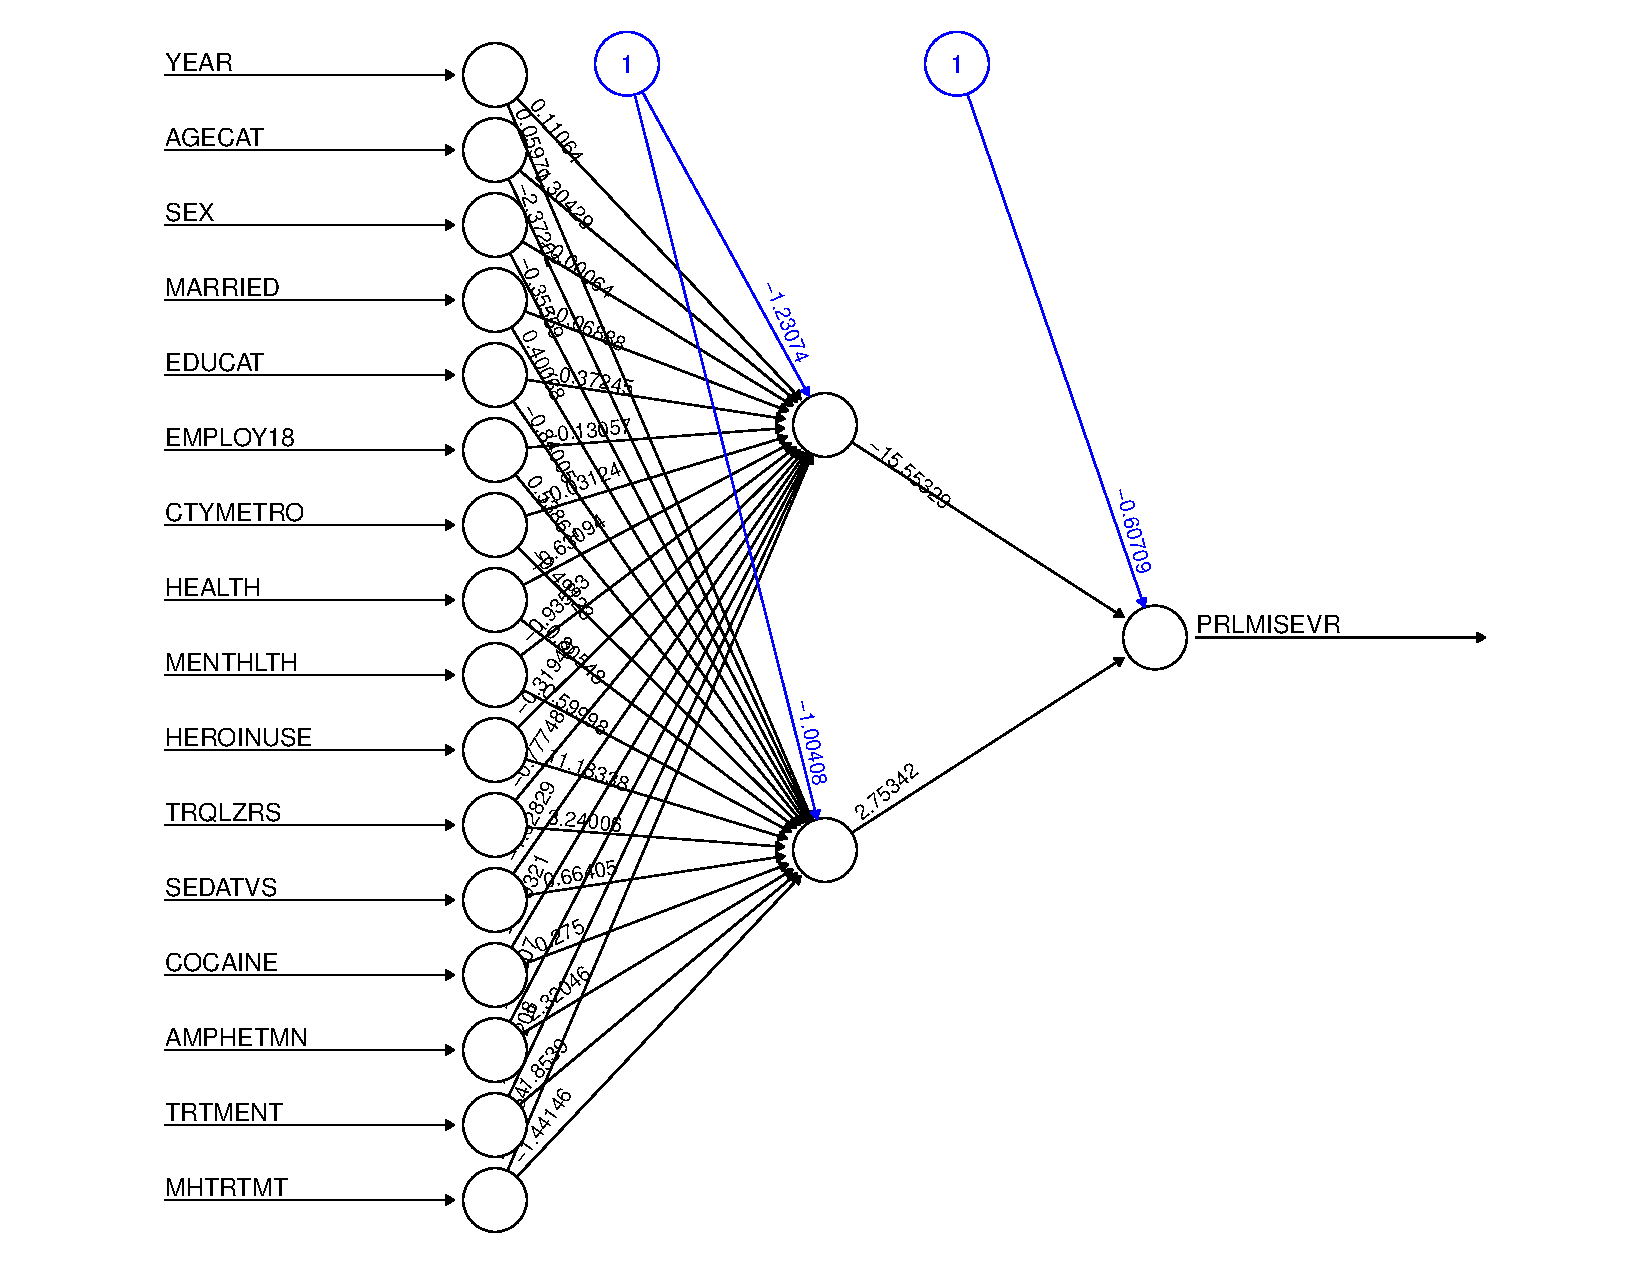
\includegraphics[width=\columnwidth]{images/Figure5.pdf}
  \caption{Proportion of Individuals Reporting Pain Reliever Misuse and Abuse
  and Heroin Use Ever as a function of Sex}
  \label{f:Figure5}
\end{figure}

%%%%%%%%%%%%%%%%%%%%%%%%%%%%%%%%%%%%%%%%%%%%%%%%%%%%%%%%%%%%%%%%%%%%%%%%%%%%%%%%

\subsection{Comparison of Classifier Models}

Model performance was evaluated and reported in the confusion matrix (Table 3), 
which include metrics of Accuracy (percentage), Sensitivity (i.e., Recall), 
Precision, and the $f_1-score$. 

 

 
%%%%%%%%%%%%%%%%%%%%%%%%%%%%%%%%%%%%%%%%%%%%%%%%%%%%%%%%%%%%%%%%%%%%%%%%%%%%%%%%
 
\begin{table*}[ht]
  \caption{Confusion Matrices and Performance Metrics for Predictive Models of 
  Pain Reliever Misuse and Abuse}
  \label{tab:freq}
  \begin{tabular}{llllllll}
    \toprule
    Model& & Confusion Matrix & & Accuracy & Sensitivity & Precision & F1-Score \\
    \midrule
    K-Nearest Neighbors & & No Misuse & PRL Misuse &  &  &  & \\
     & No Misuse & 25114 & 320 & 89.5\% & 0.900 & 0.870 & 0.870 \\
     & PRL Misuse & 2609 & 467 &  &  &  & \\
    \midrule
    Logistic Regression & & No Misuse & PRL Misuse &  &  &  & \\
     & No Misuse & 25002 & 2509 & 90\% & 0.986 & 0.909 & 0.946 \\
     & PRL Misuse & 344 & 654 &  &  &  & \\
    \midrule
    Linear Discriminant Analysis (LDA) & & No Misuse & PRL Misuse &  &  &  & \\
     & No Misuse & 24668 & 2239 & 89.8\% & 0.973 & 0.917 & 0.944 \\
     & PRL Misuse & 678 & 924 &  &  &  & \\
    \midrule
    Quadratic Discriminant Analysis (QDA) & & No Misuse & PRL Misuse &  &  &  & \\
     & No Misuse & 23165 & 1780 & 86.1\% & 0.914 & 0.9929 & 0.921 \\
     & PRL Misuse & 2181 & 1383 &  &  &  & \\
    \midrule
    Support Vector Classifier (SVC) & & No Misuse & PRL Misuse &  &  &  & \\
     & No Misuse & 25201 & 233 & 90.4\% & 0.900 & 0.890 & 0.880 \\
     & PRL Misuse & 2514 & 562 &  &  &  & \\
    \midrule
    Naive Bayes Classifier & & No Misuse & PRL Misuse &  &  &  & \\
     & No Misuse & 25345 & 3133 & 89\% & 0.999 & 0.890 & 0.941 \\
     & PRL Misuse & 1 & 30 &  &  &  & \\
    \midrule
    Neural Network (MLP) & & No Misuse & PRL Misuse &  &  &  & \\
     & No Misuse & 25088 & 346 & 90.6\% & 0.910 & 0.890 & 0.880 \\
     & PRL Misuse & 2366 & 710 &  &  &  & \\
    \midrule
    Decision Trees & & No Misuse & PRL Misuse &  &  &  & \\
     & No Misuse & 25042 & 2572 & 89.9\% & 0.988 & 0.907 & 0.946 \\
     & PRL Misuse & 304 & 591 &  &  &  & \\
    \midrule
    Random Forests & & No Misuse & PRL Misuse &  &  &  & \\
     & No Misuse & 25026 & 2298 & 90.1\% & 0.987 & 0.909 & 0.946 \\
     & PRL Misuse & 320 & 665 &  &  &  & \\
    \midrule
    Gradient Boosted Trees & & No Misuse & PRL Misuse &  &  &  & \\
     & No Misuse & 25415 & 19 & 89.6\% & 0.900 & 0.890 & 0.850 \\
     & PRL Misuse & 2954 & 122 &  &  &  & \\
    \bottomrule
  \end{tabular}
\end{table*}

%%%%%%%%%%%%%%%%%%%%%%%%%%%%%%%%%%%%%%%%%%%%%%%%%%%%%%%%%%%%%%%%%%%%%%%%%%%%%%%%

\subsubsection{Logistic Regression}
 
This analysis used logistic regression to predict pain reliever misuse and abuse
from the set of predictor variables. The logistic regression classifier was fit to 
the training data using the caret package, and the model was validated on the test 
data. Together, all of the variables entered into the model significantly predicted 
pain reliever misuse and abuse; only mental health treatment was a non-significant
predictor. Table 4 provides the parameter estimates for the predictor variables 
sorted in descending order by z-score, which gives an indication of the relative
influence of each predictor on the outcome variable. The logistic regression model 
identified cocaine, amphetamines, tranquilizers, mental health, age category, and 
heroin use as six of the most influential predictors of pain reliever misuse and 
abuse. The model was rerun leaving out the non-significant variables, mental health treatment, which did not change the sign or significant of the parameter estimates. 
Age category, sex, and size of city of metropolitan area were negatively related
to the outcome variables, whereas the remaining significant predictors were 
positively related to pain reliever misuse and abuse


%%%%%%%%%%%%%%%%%%%%%%%%%%%%%%%%%%%%%%%%%%%%%%%%%%%%%%%%%%%%%%%%%%%%%%%%%%%%%%%%

\begin{table}
  \caption{Coefficient Estimates for Logistic Regression Model 
  of Pain Reliever Misuse and Abuse fit to the Training Set}
  \label{tab:freq}
  \begin{tabular}{llll}
    \toprule
    Predictor&  Estimate& Std. Error& z-value  \\    
    \midrule
    (Intercept)& -2.960 &   0.048 & -61.10 ***  \\
    COCAINE  &    0.690 &   0.019 &  36.91 ***  \\
    AMPHETMN &    0.608 &   0.021 &  29.92 ***  \\
    TRQLZRS  &    0.381 &   0.014 &  27.29 ***  \\
    MENTHLTH &    0.136 &   0.006 &  22.42 ***  \\
    AGECAT   &   -0.216 &   0.013 & -16.75 ***  \\
    HEROINUSE&    0.798 &   0.052 &  15.47 ***  \\  
    EMPLOY18 &    0.222 &   0.016 &  13.72 ***  \\
    TRTMENT  &    0.195 &   0.019 &  10.47 ***  \\
    SEDATVS  &    0.281 &   0.029 &   9.63 ***  \\   
    HEALTH   &    0.103 &   0.012 &   8.27 ***  \\
    EDUCAT   &    0.104 &   0.013 &   8.22 ***  \\   
    SEX      &   -0.186 &   0.026 &  -7.24 ***  \\
    CTYMETRO &   -0.068 &   0.013 &  -5.03 ***  \\
    MARRIED  &    0.051 &   0.012 &   4.10 ***  \\
    MHTRTMT  &   -0.024 &   0.018 &  -1.32     \\
    \bottomrule
    Note: *** p-value $<$ 0.001. &  &  
  \end{tabular}
\end{table}

%%%%%%%%%%%%%%%%%%%%%%%%%%%%%%%%%%%%%%%%%%%%%%%%%%%%%%%%%%%%%%%%%%%%%%%%%%%%%%%%

\subsubsection{Decision Tree Classifier}

The following analysis used the \emph{Decision Tree Classifier} package in 
Scikit-Learn, which only does pre-pruning. First, the decision model was build
using the default setting of a fully developed tree until all leaves are pure. 
The random state` features is fixed to break ties internally. Accuracy on the
training set was 0.99 and test set accuracy was 0.974. Without restricting 
their depth, decision trees can become complex; unpruned trees are prone to 
overfitting and do not generalize well to new data. Limiting the depth of 
tree decreases overfitting, which results in lower training set accuracy, 
but improved performance on the test set. 

Next, pre-pruning was applied, with 
a maximum depth of 4, which means the algorithm split on four consecutive
questions. Training set accuracy of the pruned tree was 0.985 and test set
accuracy was 0.984. Even with a depth of 4, the tree can become a bit complex.
Figure 5 shows a partial view of the decision tree classifier of heroin use 
(the entire tree was too wide to include as a legible Figure), and the full 
tree image is available in the notebook BDA-Analytics-Classifier-Heroin.ipynb 
\cite{classifyH}. 

One way to interpret a decision tree it by following the sample numbers 
represented at the test split for each node. The classifier algorithm 
selected Cocaine Use (aggregated score) as the root node of the decision tree. 
The branch to the left  side of the tree represents samples with a score equal 
to or less than 1.5 (n=40956), whereas the branch to the right represents 
samples with a Cocaine Use score greater than 1.5 (n=1903). The second split 
on the right occurs for X, with n=1443 having a score less than or equal 
to 3.5, and n=460 respondents with a PRL score greater than 3.5. In other 
words, of those respondents who reported relatively high Cocaine use, a small
portion also reported relatively high Prescription Opioid PRL use. Instead of 
looking at the whole tree, feature importance is a common summary function 
that rates how important each feature is for the classification decisions 
made in the algorithm. 

Each feature is assigned an importance value between 0 and 1; with a value of 
1 indicating the feature perfectly predicts the target and a value of 0 meaning 
that the feature was not used at all. Feature importance values also always 
sum to 1. A feature may have a low importance value because another feature 
encodes the same information. 

The top two important features for classifying Heroin Use were Cocaine Use 
and Any Prescription Opioid PRL Use, with smaller importance given to Opioid 
PRL Misuse Ever and Prescription Opioid PRL Misuse and Abuse. 



As Figure 9 shows, the decision tree classifier
selected Cocaine Use as the root note, that branched by the test score equal
to or less than 0.5 (any Cocaine Use). At the second node, on the branch to 
the right n=5015 samples were further divided according to heroin use, with 
n=1913 having a score greater than 0.5 (any Heroin Use). At the third node
on the right branch, samples were selected according to Tranquilizer
medication use, with n=1419 scoring positively. On the left branch, the 
second node selected was Drug Treatment, with n=2844 respondents scoring
positively that they had received Drug Treatment. Feature importance of
the decision tree classifier selected Cocaine Use as the most informative
feature for Prescription Opioid PRL Misuse. Following afterwards, 
Tranquilizer Use, Drug Treatment, and Heroin Use were tied for second place. 

\begin{figure}[!ht]
  \centering\includegraphics[width=\columnwidth]{images/Figure6.pdf}
  \caption{Decision Tree Classification of Pain Reliever Misuse and Abuse}
  \label{f:Figure6}
\end{figure}


%%%%%%%%%%%%%%%%%%%%%%%%%%%%%%%%%%%%%%%%%%%%%%%%%%%%%%%%%%%%%%%%%%%%%%%%%%%%%%%%
\subsubsection{Random Forests Classifier}

 The important parameters for the random forests algorithm are 
the number of sampled data points and the maximum number of features; 
the algorithm could look at all of the features in the dataset or a limited 
number. A high value for \emph{maximum-features} will produce trees in the 
random forest that are very similar and will fit the data easily based on the most distinctive features, whereas a low value will 
produce trees that are very different from each other, and reduces over-
fitting. 


Random forests is an ensemble approach that builds many trees and averages 
their results to reduce overfitting. 

The model was build using the 
\emph{Random Forest Classifier} package in Scikit-Learn. The parameters of 
interest for building random forests are: (a) the number of trees 
(n-estimators), (b) the number of data points for bootstrap sampling 
(n-samples), and (c) the maximum number of features considered at each node 
(max-features). 

The max-features parameter determines how random each tree is, 
with smaller values of max-features resulting in trees in the random forest 
that are very different from each other. This analysis applied a random forest 
consisting of 100 trees 

The test set accuracy was 0.984. 
Often the default settings for random forests work well, but we can apply
pre-pruning as with a single tree, or adjust the maximum number of features. 
Feature importance for random forests is computed by aggregating the feature 
importance over trees in the random forest, and random forests gives
non-zero importance to more features than a single tree. 

The Random Forest Classifier package in Scikit-Learn was used to classify
Prescription Opioid PRL Misuse as the target variable, with 100 trees. The 
model accuracy for the training set was 0.955 and the test set accuracy was 
0.896, which suggests that the model overfit the data. 


compensating for some of their shortcomings of overfitting.

Although random forests models are more accurate than a single tree and can
compensate for some of the shortcomings of overfitting, a limitation of this 
approach is that it can be difficult to interpret an ensemble of trees apart 
from the measure of feature importance provided in the output. Single trees 
are still useful for visually representing the decision process.

%%%%%%%%%%%%%%%%%%%%%%%%%%%%%%%%%%%%%%%%%%%%%%%%%%%%%%%%%%%%%%%%%%%%%%%%%%%%%%%%
\subsubsection{Gradient Boosting Classifier Tree}


This analysis used the 
\emph{Gradient Boosting Classifier} from Scikit-Learn to classify Heroin Use, 
with the default setting of 100 trees of maximum depth of 3, and a learning 
rate of 0.1. The model was build on the training set and evaluated on the test 
set, with both training set and test set accuracy equal to 0.984. To reduce
overfitting, pre-pruning could be implemented by reducing the maximum depth, 
or by reducing the learning rate. Figure 7 shows that the feature importance 
for the gradient boosting classifier tree looks similar to the feature 
importance for random forests, but the gradient boosting has decreased the 
importance of many features to zero. Again Cocaine is selected as the most 
imformative features, followed by Any Opioid PRL Use. In addition to 
Prescription Opioid PRL Misuse and Abuse, the gradient boosting classifier 
selected Amphetamine Use as an informative feature of Heroin Use. 

\begin{figure}[!ht]
  \centering\includegraphics[width=\columnwidth]{images/Figure7.pdf}
  \caption{Neural Net Classifier: Multilayer Perceptron with Single Hidden Layer}
  \label{f:Figur7}
\end{figure}

The Gradient Boosting Classifier from Scikit-Learn was used to classify 
Prescription Opioid PRL Misuse, using the default setting of 100 trees, of 
maximum depth of 3, and a learning rate of 0.1. The model accuracy for the
training set was 0.894 and accuracy for the test set was 0.893. Gradient 
boosting typically improves test set accuracy by using many simple models 
iteratively. In this case, model accuracy for gradient boosting was no better 
than random forests, and this is because the default parameter settings were
used; further parameter tuning is needed to improve model performance. Feature 
importance was a primary interest for identifying features related to '
prescription opioid abuse. Figure 11 shows the feature importance for the 
gradient boosting classifier tree. As Figure 11 shows, several features were 
important for classifying prescription opioid misuse, and contrary to the 
random forests, gradient boosting selected Tranquilizer use as the most 
informative feature. Following closely in importance were Heroin Use and Age 
Category. Tied for fourth place were Cocaine Use and Treatment, with Mental 
Health (depression) coming in fourth in terms of feature importance. This 
result illustrates that several features are important for understanding 
Prescription Opioid Misuse, and the relations among features may be complex.

%%%%%%%%%%%%%%%%%%%%%%%%%%%%%%%%%%%%%%%%%%%%%%%%%%%%%%%%%%%%%%%%%%%%%%%%%%%%%%%%

\subsubsection{Tradeoff Between Accuracy and Interpretability}

One of the simplest classifier algorithms, K-Nearest Neighbors (KNN)
classifies a new data point based on the Euclidean distance to its 
nearest neighbors and provides a solution that is easy to understand. 
However, KNN does not perform well with a large number of features 
(100 or more) or sparse datasets.

SVMs often perform well, but are sensitive to parameter settings 
and scaling of the data. 

%%%%%%%%%%%%%%%%%%%%%%%%%%%%%%%%%%%%%%%%%%%%%%%%%%%%%%%%%%%%%%%%%%%%%%%%%%%%%%%%

\section{DISCUSSION}

% Summarize main findings

The results show that rates of prescription opioid use, misuse, and abuse are
much higher than use of illicit opioids such as heroin and fentanyl. The use 
of Hydrocodone (Vicodan) was double the rate of Oxycodone use (Oxycodone) 
across almost all age groups. The use of traditional prescription opioids 
was greater than reported use of synthetic opioids. Illicit drug use was 
highest for respondents between the ages of 18 to 25. In terms of mental 
health, more individuals between 18 to 25 years reported experiencing a major 
depressive episode (in adulthood) than any other age group. 

The large majority of respondents (89\$ percent) had not misused 
prescription opioid 
pain relievers or used heroin. 

Of those individuals who reported 
misusing prescription opioid pain relievers, almost twice as many had also
used heroin than had not (see Figure 1), which partially supports the 
hypothesis that prescription opioid use is associated will use of illicit 
opioids such as heroin. 
 
 Recent statistics from the CDC show that heroin use
has increased among most demographics groups, with an average estimated rate 
of approximately 2.6 percent between 2011-2013 \cite{cdc16}.

The rate of heroin use reported in the NSDUH-2015 sample was 1.6 percent. 
Therefore, it seems that the actual rate of heroin use in the U.S. population 
may not be accurately reflected in this sample. 

 
%%%%%%%%%%%%%%%%%%%%%%%%%%%%%%%%%%%%%%%%%%%%%%%%%%%%%%%%%%%%%%%%%%%%%%%%%%%%%%%%

\subsection{Comparison of Classifier Models}

Several classifier algorithms were used to identify relevant features for 
predicting heroin use and prescription opioid misuse. Comparing the performance 
of different algorithms is helpful for  selecting the best model. 

Test set
accuracy was comparable across models for both Heroin Use (0.98) and 
Prescription Opioid PRL Misuse (0.89-0.90). Logistic Regression provided the
feature coefficients for different values of the regularization parameter C. 
The Decision Tree classifier provided a easy to use, interpretable visual of
the decisions involved at each step of classification. Random forests provides
a more reliable indication of features importance than a single tree, 
whereas the gradient boosting classifier included additional tuning 
parameter for a more powerful model and more interpretable analysis of
feature importance. 

Each classifier method provides a different level of
analysis. 
logistic regression showed that Treatment had the highest coefficient value, but 
the tree based models each differed in selecting the most important features. 

Decision trees indicated that Cocaine Use was most informative, the random 
forests classifier selected health as the most important feature, and the 
gradient boosting model selected 
Tranquilizer use as most informative of prescription opioid PRL misuse. 

The different models each have their advantages and limitations, logistic regression provides the coefficients, but random forests and gradient boosting are helpful for 
identified sets of important features.

%%%%%%%%%%%%%%%%%%%%%%%%%%%%%%%%%%%%%%%%%%%%%%%%%%%%%%%%%%%%%%%%%%%%%%%%%%%%%%%%
\subsection{Combine Limitations and Extensions}

Surveys data may be biased to some degree, but measures of confidentiality and 
anonymity help to assure more accurate disclosures. 

The main goal of this project was to 


identify features relevant for predicting 
opioid addiction by classifying cases according to heroin use. 

A limitation of survey data is that responses may be biased by under-reporting or minimizing the use of illicit or illegal substances. People may also be reluctant to disclose mental health issues or health problems (e.g., STDs, HIV status, suicide attempts). 

It is possible that this sample is representative of the frequency of opioid use 
and misuse in the larger population.


A limitation is that the project dataset was constructed as a subset of 
features from the NSDUH-2015 data. 
Ninety attributes were selected out of 2666 features in the original dataset, 
and many features were combined to create aggregated variables for health, 
mental health, prescription opioid misuse and abuse, drug treatment, mental health
treatment. 

Future research could include a more comprehensive selection of
features to identify the set of features relevant for predicting opioid
dependency and addiction. 


%%%%%%%%%%%%%%%%%%%%%%%%%%%%%%%%%%%%%%%%%%%%%%%%%%%%%%%%%%%%%%%%%%%%%%%%%%%%%%%%
\subsection{Extension to Big Data}

The methods used in this project could be extended to better approximate big 
data for predicting opioid use in the following ways: (1) Include a larger 
selection of features from the attributes in the NSDUH-2015 dataset; (2) 
Include survey data from previous years (e.g., 2005-2015) for a larger sample;  
and (3) Obtain a broader sample from the population of patients who are 
taking prescribed opioid medications. The most immediate step would be to 
include additional features for use with the classifier models. Additional 
data from the NSDUH was downloaded from previous years (2012 to 2014); 
preliminary examination of the data revealed inconsistencies in questions 
and prescription opioid medications that would need to be resolved in order 
to combine data from multiple years. Data cleaning can be a time consuming 
process, but important for obtaining usable data. Unfortunately, owing to 
constraints of time for completing the project, it was not possible to
integrate data from previous years into the project dataset. In working with
big data, there are there are several steps involved in the consolidation of 
data from multiple sources into a single dataset (in addition to data 
cleaning), which include extraction, integration, and aggregation of features  
\cite{rahm00}. A future study could integrate data from different years, 
using a broader set of features, with more inclusive sample representative
of the larger population, and integrate data from multiple sources. 

%%%%%%%%%%%%%%%%%%%%%%%%%%%%%%%%%%%%%%%%%%%%%%%%%%%%%%%%%%%%%%%%%%%%%%%%%%%%%%%%
\subsection{Opioid Addiction Epidemic}

If the crisis of opioid addiction were an epidemic like other illnesses caused 
by biological contagion, its spreading or diffusion could be measured by the 
proportion of infected in the population, those yet to be infected, and the 
rate of transmission. Although drug addiction has many similar characteristics 
to other chronic medical illnesses, but there are unique challenges to the 
treatment of addiction \cite{marsch12, swendson16}. According to the classical 
conditioning theory of addiction, situational cues or events can elicit a 
motivational state underlying the relapse to drug use. Following treatment, 
many addicted individuals return to the same environments associated with 
their drug use. Addictive behavior can be reinstated by exposure to drug-
related cues or stressors in the environment \cite{shaham03}, putting
individuals in recovery at risk for relapse and possible overdose \cite{johnson11}. 
Furthermore, the structure of social contact networks can influence epidemic 
spreading or diffusion \cite{pastor01, watts98}, as person-to-person contact 
and indirect associations may facilitate the spread of drug use and addictive 
behavior. In the case of prescription opioids, anyone is potentially at 
risk of misusing opioids and becoming addicted. Rather than labeling people 
as addicted or not addicted, it may be useful to consider people as more or 
less susceptible to misusing or abusing opioid pain medication, leading to
a greater or lesser susceptability to becoming dependent or addicted to 
opioids. 

%%%%%%%%%%%%%%%%%%%%%%%%%%%%%%%%%%%%%%%%%%%%%%%%%%%%%%%%%%%%%%%%%%%%%%%%%%%%%%%%
\section{Conclusion}

The present study compared the results of several classification models of 
pain reliever misuse and abuse. A general conclusion is that 

The results do not provide sufficient evidence to rule out alternative hypotheses. 

Several features were identified as important for classifying pain reliever
misuse and abuse, including Cocaine Use, Amphetamine Use, tranquilizer use,
age category, overall health,

Prescription opioid misuse and abuse was associated with heroin use: of 
the individuals who reported misusing prescription opioid medications, twice 
as many reported having used heroin than those who said that they had not used 
heroin. the importance of heroin use was a predictor of pain reliever misuse and
abuse was limited, given the very small number of individuals who reported 
using heroin.

additional evidence is needed to address these question. 

Predictive modeling is a useful approach for classifying individuals as 
having misused or abuse opioid pain relievers and may help inform 
efforts to address the opioid crisis and reduce risk of overdose deaths. 


%%%%%%%%%%%%%%%%%%%%%%%%%%%%%%%%%%%%%%%%%%%%%%%%%%%%%%%%%%%%%%%%%%%%%%%%%%%%%%%%
\begin{acks}

Portions of this paper were completed as part of a course project in Big Data 
Applications and Analytics taugt by Dr. Gregor von Laszewskin at Indiana 
University in the Fall 2017. Thanks to the Professor von Laszewski and the
Teaching Assistants, Juliette Zurick, Miao Jiang, Hungri Lee, Grace Li, and 
Saber Sheybani Moghadam for helpful comments and feedback.

\end{acks}

\bibliographystyle{unsrt} %%ACM-Reference-Format%%
\bibliography{report} 


%%%%%%%%%%%%%%%%%%%%%%%%%%%%%%%%%%%%%%%%%%%%%%%%%%%%%%%%%%%%%%%%%%%%%%%%%%%%%%%%
\appendix

\section{Code References}
All code, notebooks, files, and folders for this project can be found in the

%%%%%%%%%%%%%%%%%%%%%%%%%%%%%%%%%%%%%%%%%%%%%%%%%%%%%%%%%%%%%%%%%%%%%%%%%%%%%%%%


%\input{issues}

\end{document} 
